%%%%%%%%%%%%%%%%%%%% author.tex %%%%%%%%%%%%%%%%%%%%%
%%%%%%%%%%%%%%
%
% sample root file for your "contribution" to a contributed volume
%
% Use this file as a template for your own input.
%
%%%%%%%%%%%%%%%% Springer %%%%%%%%%%%%%%%%%%%%%%%%%
%%%%%%%%%


% RECOMMENDED %%%%%%%%%%%%%%%%%%%%%%%%%%%%%%%%%%%%
%%%%%%%%%%%%%%%
\documentclass[graybox]{svmult}

% choose options for [] as required from the list
% in the Reference Guide

\usepackage{mathptmx}       % selects Times Roman as basic font
\usepackage{helvet}         % selects Helvetica as sans-serif font
\usepackage{courier}        % selects Courier as typewriter font
\usepackage{type1cm}        % activate if the above 3 fonts are
                            % not available on your system
%
\usepackage{makeidx}         % allows index generation
\usepackage{graphicx}        % standard LaTeX graphics tool
                             % when including figure files
\usepackage{multicol}        % used for the two-column index
\usepackage[bottom]{footmisc}% places footnotes at page bottom
%\usepackage{subcaption} %% ADDED
%%% Personal packages
%\usepackage[utf8]{inputenc}
\usepackage{longtable}
\usepackage{color}
\usepackage{multirow}
% see the list of further useful packages
% in the Reference Guide

\makeindex             % used for the subject index
                       % please use the style svind.ist with
                       % your makeindex program

%%%%%%%%%%%%%%%%%%%%%%%%%%%%%%%%%%%%%%%%%%%%%%
\newcommand{\TODO}[1]{\begingroup\color{red}#1\endgroup}

%%%%%%%%%%%%%%%%%%%%%%%%%%%%%%%%%%%%%%%%%%%

\begin{document}
\tableofcontents

\title*{non-protein-coding RNAs as regulators of development in tunicates}

% Use \titlerunning{Short Title} for an abbreviated version of
% your contribution title if the original one is too long
\author{Cristian A. Velandia-Huerto, Federico D. 
Brown, Adriaan A. Gittenberger, Peter F. Stadler and Clara I. 
Berm\'{u}dez-Santana}

% Use \authorrunning{Short Title} for an abbreviated version of
% your contribution title if the original one is too long

\institute{C.A. Velandia-Huerto, \at Bioinformatics Group, Department of 
Computer Science, and Interdisciplinary Center for Bioinformatics, 
Universit{\"a}t Leipzig, H{\"a}rtelstra{\ss}e 16--18, D-04107, Leipzig, 
Germany
\at Biology Department, Universidad Nacional de Colombia, Carrera 45 \# 26-85, 
Edif. Uriel Guti{\'e}rrez, Bogot{\'a}, 
Colombia, \email{cristian@bioinf.uni-leipzig.de}.
\and F.D. Brown, \at Departamento de Zoologia, Instituto Bioci{\^e}ncias, 
Universidade de S{\~a}o Paulo, Rua do Mat{\~a}o, Tr. 14 no. 101, S{\~a}o Paulo, 
SP, Brazil
\at Laboratorio de Biolog{\'i}a del Desarrollo Evolutiva, 
Departamento de Ciencias Biol{\'o}gicas, Universidad de los Andes, Cra 1 
No. 18A-12, Bogot{\'a}, Colombia, \email{fdbrown@usp.br}.
A.A. Gittenberger, \at Institute of Biology, Leiden University, P.O. 
Box 9505, 2300 RA, Leiden, Netherlands 
\at GiMaRIS, BioScience Park Leiden, J.H. Oortweg 21, 2333 CH, Leiden, 
Netherlands
\at Naturalis Biodiversity Center, Darwinweg 2, 2333 CR,Leiden, Netherlands,
\email{gittenberge@gimaris.com}.
\and P.F. Stadler, \at Bioinformatics Group, Department of Computer Science, 
and Interdisciplinary Center for Bioinformatics, Universit{\"a}t 
Leipzig, H{\"a}rtelstra{\ss}e 16--18, D-04107, Leipzig, Germany, 
\email{studla@bioinf.uni-leipzig.de}.
\and C.I. Berm\'{u}dez-Santana, \at Biology Department, Universidad 
Nacional de Colombia, Carrera 45 \# 26-85, Edif. Uriel Guti{\'e}rrez, 
Bogot{\'a}, Colombia, \email{cibermudezs@unal.edu.co}.
}

%
% Use the package "url.sty" to avoid
% problems with special characters
% in your e-mail or web address
%
\maketitle


\abstract{Tunicates, or urochordates, are a group of small marine organisms
  that are found found widely throughout the seas of the world. As most
  plausible sister group of the vertebrates they are of utmost importance
  for a comprehensive understanding of chordate evolution, hence they have
  served as model organisms for many aspects of the developmental biology.
  Current genomic analysis of tunicates indicates that their genomes
  evolved with a fast rate not only at the level of nucleotide
  substitutitions but also in terms of genomic organization. The latter
  involves genome reduction, rearrangements, as well as the loss of some
  important coding and non-coding RNA (ncRNAs) elements and even entire
  genomic regions that are otherwise well conserved. These observations are
  largely based on evidence from comparative genomics resulting from the
  analysis of well-studied gene families auch as the Hox genes and their
  non-coding elements. In this chapter the focus lies the ncRNA complement
  of tunicates, with a particular emphasis on microRNAs, which have already
  been studied extensively for other animal clades. MicroRNAs are known as
  important regulators of key genes in animal development and they are
  intimately related to the increase morphological complexity in higher
  metazoans. Here we review the discovery, evolution, and genome
  organization of the miRNA repertoire, which has been drastically reduced
  and restructured in tunicates compared to the chordate ancestor.  Known
  functions of microRNAs as regulators of development in tunicates are a
  central topic. For instance we consider the rolte of miRNAs as regulators
  of the muscle development and their importance in the regulation of the
  differential expression during the oral siphon regeneration. Beyond
  microRNAs, we touch upon the functions of some other ncRNAs such as
  Yellow Crescent RNA, moRNAs, RMST lncRNAs, or spliced-leader (SL) RNAs,
  which have diverse functions associated with the embryonic development,
  neurogenesis and mediation of mRNA stability in general.}

\section{Introduction}
\label{sec:1}

Tunicates are organisms characterized by a fast rate of genomic and
developmental evolution. Some fast evolving evolutionary changes include
loss of synteny, fast changes in cis-regulatory sequences, and loss of
several key regulatory developmental genes \cite{Satou2008, Denoeud1381},
such as several central or posterior Hox genes involved in AP patterning of
metazoans \cite{Ikuta:2005} and Gbx involved in the establishment of the
midbrain-hindbrain boundary in vertebrates \cite{Yagi2003}.

The role of noncoding RNAs in tunicate development has been studied since
the 1990's, dating back to the seminal work by Swalla \& Jeffry on the RNAs
localized in the yellow crescent or myoplasm, a cytoskeletal domain in
oocytes of the ascidian \textit{Styela clava} \cite{Swalla1995}. The yellow
crescent (YC) RNA identified to be present throughout embryonic development
was the first example of what his now a large and rapidly growing class of
ncRNAs with important roles in growth and development in tunicates. This
asymmetrically distributed ascidian RNAs were part of the set of many other
RNAs known as maternally synthesized cytoplasmically localized RNAs,
discovered first in oocytes of Xenopus \cite{Bashirullah1998}.

The current state of knowledge on ncRNAs in tunicates is far from
comprehensive and complete. Nevertheless, in particular microRNAs have been
studied already in some detail in several tunicates species, in particular,
\textit{Oikopleura dioica}, both Ciona species\footnote{In accordance with
  the prevalent use in the ascidian community we use the term \textit{Ciona
    robusta} reflecting that ``Morphological evidence that the molecularly
  determined \textit{C.\ intestinalis} type A and type B are different
  species: \textit{Ciona robusta} and \textit{C.  intestinalis}"
  \cite{Brunetti:2015}.}, \textit{Didemnum vexillum}, and \textit{Salpa
  thompsoni}. These studies have revealed many losses miRNA families that
are very well conserved outside the tunicates. At the same time, many gains
of unique miRNAs among recently divergent lineages in the tunicates when
compared to other groups of chordates \cite{Fu2008,
  Velandia-Huerto2016}. Relaxed constraints in the evolution of genomes and
developmental trajectories in the tunicates may have been responsible for
the plethora of reproductive strategies, morphologies, and life histories
observed in the group \cite{Holland2015}.

\section{miRNA families origin and evolutionary perspective}
\label{sec:2}

\subsection{Origins and Evolution of MicroRNAs}

MicroRNAs (miRNAs) have been described in almost all animals and plants as
well as diverse unicellular eukaryotes. They are important
post-transcriptional regulators of gene expression affecting a sizable
fraction of all mRNAs \cite{Ameres:13}. Mechanistically, miRNAs depends on
the presence of the evolutionarily even older RNA interference pathways
\cite{Cerutti:06, Shabalina:08} that leads to the suppression of
double-stranded RNA molecules in a cell's cytoplasm.

Throughout animals, canonical miRNAs are the processed through a
well-characterized pathway. The primary precursor transcript (pri-miRNA) is
transcribed by pol-II. While in most cases the pri-miRNA is a long
noncoding RNA, some miRNAs are processed from protein-coding transcripts,
where they are mostly derived from introns \cite{Lin:06}. In the next step,
hairpin-shaped precursors, the pre-miRNAs, are extracted while the RNA is
still residing in the nucleus. These are exported into the cytoplasm
\cite{Lund:04} and then processed further into miRNA/miRNA* duplexes. In
the final step the single-stranded mature miR or its complement, the miR*,
is incorporated in RISC complex. Sequence complementarity of miR and mRNA
ensures the targeting specificity \cite{Bartel:13}. As as a consequence,
miRNAs share a set of structural characteristics, most importantly the
extremely stable secondary structure of the precursor hairpin and the 2-bp
overhang of miR and miR* generated by Dicer processing. These features make
it possible to reliably identify miRNAs from short RNA-seq data, see e.g.
\cite{Langenberger:10a, Friedlaender:12, Langenberger:13a}.

Most animal microRNAs are among the most highly conserved genetic elements.
The most stringent selection pressure acts on the mature miR sequence. This
is a consequence of the fact that a single miR typically targets a large
number of mRNAs. Mutations in the mature sequence thus simultaneous affect
many interactions, and thus are almost always selected against. In
conjunction with the stringent requirements on the secondary structure, the
entire precursor is under strong stabilizing selection \cite{Price:11},
explaining the observed high levels of sequence conservation. As a
consequence, even evolutionarily distant homologs of miRNAs can be readily
detected despite the short sequence length. Most efficiently,
\texttt{infernal} \cite{Nawrocki:13} is used for this purpose, since it
makes use of both sequence and structure comparison. The evolution of
miRNAs can thus be traced back in time with high accuracy \cite{Hertel:06a}. 

Like other gene families, miRNAs form paralogs \cite{Tanzer:04a, Hertel:12a}
and hence often appear as families as homologous genes. This forms the
basis of the \texttt{miRBase} nomenclature \cite{Ambrose:03a}. A series of
investigations into the phylogenetic distribution of miRNA families showed
that miRNAs are infrequently lost at family level and thus serve as
excellent phylogenetic markers \cite{Sempere:06, Heimberg:08, Heimberg:10, 
Wheeler:09}, although the massive restructuring of the miRNA complement of 
tunicates is an important exception to this rule \cite{Fu:08}.

The innovation of new miRNA families is an on-going process. Experimental
surveys of the miRNA repertoir thus have reported a large number of very
young and even species-specific miRNAs \cite{Bentwich:05, Berezikov:06}. The
process was studied quantitatively in fruit flies, where innovation rate of
as many as $12$ new miRNA genes per million years has been estimated
\cite{Lu:08}. This is consistent with the fact that stable hairpins are
abundant structural elements in random RNAs, which makes is not only
possible but actually quite likely that miRNA precursors appear by chance
in transcribed genomic regions \cite{Tanzer:04a, CampoPaysaa:11, Marco:13}.
Of course, only a tiny fraction of these fortuitously processed hairpins
have a function and hance are subject to selection, and an even smaller
subset is conserved over long evolutionary time scales. Detailed studies
showed that evolutionarily young miRNA have comparably low expression
levels. Initially, they go through a phase of relatively fast sequence
evolution \cite{Liang:09, Meunier:12}, which slows down as the selective
pressures from a gradual increase in the number of target site increases. A
large, diverse set of targets then protects against miRNA loss
\cite{Lee:07a}. The rate of gain of miRNA families that retained
essentially permanently amounts to only $1$ per several million years. This
number is consistent with divergence of the miRNA complements between
animal phyla.

Many authors have observed that overall the miRNA repertoire has been
expansing throughout animal evolution in a manner that at least roughly
correlates with morphological complexity \cite{Hertel:06a, Sempere:06,
  Niwa:07, Prochnik:07, Lee:07a, Heimberg:08, Peterson:09,
  Berezikov:11}. Several bursts of miRNA innovation have been observed
\cite{Hertel:06a, Heimberg:08, Tanzer:10a, Hertel:15a}, most notably at the
root of the placental mammals, the ancestor of ``free-living'' nematodes,
or the radiation of the drosophilids.  Massive morphological
simplification, on the other hand, is sometimes associated with a drastic
loss of miRNA families. This has been observed most prominently for
tunicates \cite{Fu:08, Dai:09}.

\subsection{miRNA identification and validation}

The first miRNA reported in any tunicate was let-7, which was 
first detected in \textit{Ciona robusta} and \textit{Herdmania curvata} 
\cite{Pasquinelli2000}. A previous study the same year in \textit{C.\ elegans} 
had shown that small RNA let-7 ($21$ nt) was required for late larval to adult 
developmental transition \cite{Reinhart:2000mz}. Small RNA let-7 was then shown 
to also be differentially expressed during the development of many distantly 
related animal taxa, but was not detected in Porifera, Ctenophora, Cnidaria, 
and Acoelomorpha, suggesting that let-7 was involved in the regulation of late 
temporal transitions during development or in the evolution of complex life 
histories in the Nephrozoa \cite{Pasquinelli2000,Pasquinelli2003}.

The first systematic computational screen of a tunicate genome in 2005
followed the first large animal sequencing projects. Beginning with
\textit{C.\ robusta} and \textit{C.\ savignyi}, a profile-based strategy
was implemented in the ERPIN program \cite{Legendre2005}. This work
detected a set of new miRNAs candidates considered as \textit{C.\ robusta}
specific, such as the members of the family miR-9 and miR-79 together with
many other miRNA families that, as expected, were found to be homologous between
both Ciona speces. Among these were miR-124, miR-92, miR-98, miR-325, 
the miR310-313 group, and let-7. In the same year, a whole-genomic comparative
approach in the urochordate lineage was performed on the species
\textit{C.\ robusta}, \textit{C.\ savignyi}, and \textit{O.\ dioica}. Using a
computational screening of structured ncRNAs based upon homology between
predicted precursor hairpin structures $41$ miRNA candidates were detected
including let-7 and other six known candidates in \textit{C.\ robusta}
\cite{Missal2005}. After all, the same group in 2007 implemented a
structure-based clustering approach in \textit{C. robusta} predicted $58$
miRNAs, of which only let-7, miR-7, miR-124, and miR-126 coincided with the
previously annotated miRNAs \cite{Will2007}.

Up to this point in time, efforts to map the miRNAs in urochordate lineages
were mainly focused on computational approaches. With improved sequence
technologies, new hybrid strategies were employed that combined
computational and experimental studies to validate candidate families
previously detected. For instance, the first bona fide records for
\textit{C.\ robusta} miRNAs were registered in mirBase only in Release 11
based on the data reported in \cite{Norden-Krichmar2007}. This study
searched the genomes of \textit{C.\ robusta} and \textit{C.\ savignyi} for
conservation of the seed regions of the known mature miRNA sequences
compiled in the 2006 release of miRBase release. Those miRNAs were aligned
locally using the FASTA/ssearch34 program, retaining only matches with at
least 90\% identity. The characteristic hairpin structure and the relative
positioning of the mature sequences were used as additional filters. After
manual curation a set of $18$ miRNAs that appeared conserved in both Cionas
was reported. The expression of $14$ of these families, including let-7,
miR-7, and miR-126, was then confirmed by Northern blot analyses in the
adult tissue of \textit{C.\ robusta}.

Until 2008, most of the miRNAs annotations were concentrated in Cionas, but
new annotation approaches for other species in tunicates were appearing
slowly to increase then the repertory of new miRNAs families in
urochordates. The first repertory of miRNAs in tunicate beyond the Ciona
species was pubished in 2008 for the larvacean \textit{O.\ dioica}
\cite{Fu2008}. At that time the Fu \emph{et al.}\ were studying the
temporal-spatial expression patterns of conserved miRNAs in different
developmental stages of oocytes, 1-cell zygote, 2-8 cell embryons,
blastulas, gastrulas, tadpoles (in different stages) and animals from 1 to
6 days from \textit{O.\ dioica}. Small RNAs were isolated, amplified by
RT-PCR and rapid amplification of cDNA ends (RACE) of the developmental
stages, cloned and sequenced. Blast searches using the sequences of cloned
small RNA libraries were used to annotate small RNAs as miRNA
candidates. In further steps the recovered genomic flanking sequences each
side of those mapped candidates were used as input to predicted secondary
structures by mfold v3.1.\ This step was used to detect candidates that
folds like miRNA hairpins and aimed to decrease the set of false positive
potential miRNAs in \textit{O.\ dioica}. Finally, for this set of potential
candidates a developmental miRNA array dot blot analyses were performed to
detect miRNA expression. With this approach from $3066$ sequenced small RNA
clones, expression was detected for only $55$ miRNAs.  The authors
suggested that these candidates were expressed throughout the short life
cycle of \textit{O.\ dioica} showing that some of them were stocked as
maternal determinants prior to rapid embryonic development. The authors
also identified a set of sex-specific miRNAs that appeared as male/female
gonad differentiation which became apparent and was maintained throughout
spermatogenesis \cite{Fu2008}. Unexpectedly, the majority of the miRNAs
loci in \textit{O.\ dioica} were located in antisense orientations in the
host genes, in contrast to the majority of the mammalian miRNAs known at
the time.

Between the years 2009 and 2015 the majority of the studies of miRNAs in
tunicates were focused into the validation of expression of computational
predicted miRNAs in Cionas specially focused in \textit{C.\ robusta} as
model organism of tunicates or into the test of new computational
approaches as miRTRAP, miRDeep2 and miRRim2 which used next-generation
sequencing libraries of small RNAs derived from \textit{C. robusta} to
validate their algorithms.  Then by the year 2016 the first comparative
homology based search strategy let us to identify the repertory on miRNAs
and other ncRNAs in the carpet sea squirt \textit{Didemnum vexillum} with a
preliminary comparative analysis of gain and losses of miRNA families on
chordates which included the \textit{Cionas}, \textit{O. dioca} and the
colonial tunicate \textit{Botryllus schlosseri}
\cite{Velandia-Huerto2016}. By the same year, from the preliminary genome
sequence assembled for the Southern Ocean salp, \textit{Salpa thompsoni}
(Urochordata, Thaliacea) a set of miRNAs families were detected
\cite{Jue2016} and in 2017 the prediction of miRNAs families were reported
to the species \textit{Halocynthia roretzi}.  \TODO{is there a reference?
  if so add, otherwise give a source in the text.}

\subsubsection{High throughput studies of Ciona miRNAs} 

At the end of the last decade the application of next generation sequencing
technologies to sequence small RNA libraries changed the common way used to
detect expression of miRNAs in many organisms including the tunicates. This
technology became in one of the most common approaches that supported
methods like RT-PCR, microarrays or dot blotting which were previously used
to validate miRNA expression in tunicates. In 2009 small RNA libraries
prepared from various developmental stages including unfertilized eggs,
early embryos, late embryos and adults from \textit{C.\ robusta} were
assayed by high-throughput sequencing of cDNA with an Illumina 1G Genome
Analyzer. These sequencing data revealed $80$ miRNAs families in
\textit{C.\ robusta}.  Unexpectedly, a distinct species of small RNAs
processed from the distal parts of the miRNA precursor hairpins was found
to be abundantly expressed. These were termed miRNA-offset RNAs (moRs)
\cite{Shi2009}.  Later on, after extracting non-coding conserved regions of
whole genome alignments between \textit{C.\ robusta} and \textit{C.\
  savigny} a set of $12$ million sequences were computationally folded
using RNAfold and mfold. Then after combining the following criteria:
structure/sequence conservation, homology to known miRNAs, and phylogenetic
footprinting the authors detected a set of $458$ candidate sequences
\cite{Keshavan2010}. Then in order to validate those candidate, RT-PCR and
PAGE were conducted to design a custom microarray.  $244$ of the $458$
miRNA predictions were represented either in their microarray data or in
the Illumina sequences from \cite{Shi2009}, leading to an estimate of about
$300$ miRNA genes in \textit{C.\ robusta}. It is worth noting that
\cite{Keshavan2010} did not recover $39$ previously characterized miRNAs.
A novel computational strategy for the systematic, whole-genome
identification of microRNA from high throughput sequencing information was
developed in 2010 in \cite{Hendrix2010} and applied to \textit{C.\
  robusta}. This method, miRTRAP, relies on the sequence patterns produced
by mechanisms of microRNA biogenesis but also includes additional criteria
regarding the prevalence and quality of small RNAs arising from the
antisense strand and the neighboring loci. With that approach, nearly $400$
putative microRNAs loci were detected. The miRTRAP approach is depends
crucially on the depth of the small RNAs mapped to a given locus and
requires a very accurate assignment of small RNA sequences on their
relative positions along the hairpin, that is, miR/miR*, moR/moR* and loop
\cite{Hendrix2010}. A further improvement in the analysis of miRNA
sequencing data became available with miRDeep2, a revised version miRDeep
\cite{Friedlaender:12}.  It was reported to identify with an accuracy of
$98.6$\% and $99.9$\% canonical and non-canonical miRNAs in different
species. A reanalysis of the small RNA data from \cite{Shi2009} with
miRDeep2 reported $313$ known and $127$ novel miRNAs in \textit{C.\
  robusta}. In the same year the program miRRim2 \cite{Terai2012} was
applied to the \textit{C.\ robusta} genome, in which some candidates
identified from the work of \cite{Hendrix2010} and the several promising
candidates were detected.

In 2013, \cite{Kusakabe2013} investigated the expression patterns of the
cluster miR-1 and miR-133 in \textit{C.\ robusta} and in \textit{C.\
  savignyi}. RT-PCR amplification of miR-1/133 precursors were performed
and PCR products were subcloned and sequenced. Whole-mount in situ
hybridization to detect cin-miR-1/miR-133 primary transcript was performed
and LNA Northern blotting was conducted on different developmental stages.

\subsubsection{High throughput miRNA searches in other Urochordates}

Since 2016 new approximations has increased our knowledge about new
families in other tunicates thanks to the sequence of new urochordate
genomes of the species \textit{D.\ vexillum}, \textit{S.\ thompsoni} and
\textit{H.\ roretzi}. For the draft genome sequence from
\textit{D. vexillum} an homology-based computational approach was applied
\cite{Velandia-Huerto2016}.  Blast and HMMer searches were performed with
annotated small ncRNAs sequences from metazoans and hidden markov models
from RFAM\footnote{\url{http://rfam.xfam.org/}} to obtain the sort of
candidates at sequence level. Structural alignments of those sequences were
performed by infernal \cite{Nawrocki:201}, using metazoan-specific
covariance models to annotate the small ncRNAs collection, which $57$
families and $100$ loci of miRNAs were found.

For the preliminary assembled of the genome sequence for the Southern Ocean
salp \textit{S.\ thompsoni} \cite{Jue2016} were small RNA libraries
constructed to be sequenced on an Illumina Hiseq 2000. After filtering data
sets to 18-24 nt for miRNA and 28-32 nt for piRNA, the reads were aligned
to \textit{S. thompsoni} genome and miRNA gene folding predictions were
performed using RNAfold. In this initial survey of small RNAs, were
revealed the presence of known, conserved miRNAs, as well as novel miRNA
genes and mature miRNA signatures for varying developmental stages. Then in
2017, the prediction of $319$ miRNAs candidates in \textit{H.\ roretzi}
were obtained through three complementary methods. The experimental
validation suggested that more than half of these candidate miRNAs are
expressed during embryogenesis. The expression of some of the predicted
miRNAs were validated by RT-PCR using embryonic RNA. In this approach
\textit{C.\ robusta} small RNA-Seq reads derived from \textit{C.\ robusta}
\cite{Shi2009} (previously known as \textit{C. intestinalis} today
reclassified) was used to identify conserved miRNAs in \textit{H.\ roretzi}
\cite{Wang2017}.

Current repertorie of miRNAs (Figure \ref{fig:matrimirnas}) is based on the
final matrix of miRNAs families from \cite{Hertel:15a} and complemented by
homology methods developed on \ref{Velandia-Huerto2016}, specifically for
\textit{S. thompsoni} and \textit{H. roretzi} blast searches with
structural alignments where applied on the reported candidates in
\cite{Jue2016} and \cite{Wang2017}.

\TODO{begin construction}

\subsection{miRNA in clusters}

One of the most interesting aspects about the patterns of genomic locations of 
miRNAs is to known whether those loci are randomly distributed throughout the 
genome as single copies or if they are arranged on consecutive locations or in 
tandem copies clustered to be expressed from polycistronic primary precursors 
or to be transcribed independently \cite{TanzerALL:2010}. Interestingly in 
\textit{O. dioca} miRNAs are located in the antisense orientations of 
protein-coding gene and immediately downstream of its corresponding 3`UTR region 
or even more in the sense strand of introns \cite{Fu2008}. Nevertheless, after 
those conspicuous distributions some clusters have been also identified in 
\textit{O. dioca}. For instance four miRNAs, miR-1490a, miR-1493, miR-1497d, and 
miR-1504, are reported by \cite{Fu2008} to be presented as two copies, and 
miR-1497d-1 and miR-1497d-2 are included in the large miR-1497 cluster. See the 
current structure of this cluster in Table \ref{tab:detailBigClusters} although 
only one copy for the miR-1497 has been reported for \textit{C. robusta} 
located in an intergenic region \cite{Fu2008, Hendrix2010} and one in 
\textit{C. savigny} overlapped in an intron \cite{Fu2008}. By testing real time 
PCR co-expression of some miRNAs, their host and adjacent genes in \textit{O. 
dioca} by \cite{Fu2008} it was discovered for the case of the cluster  
miR-1487/miR-1488 a not clear positive or negative correlation with the 
expression of its anti-sense hosting gene. In males this cluster expression was 
not associated with the expression of its adjacent ABCA3 gene by the same 
authors.  

%%%
\begin{small}
\begin{center}
\begin{longtable}{p{2.0 cm}p{2 cm}p{2 cm}p{2 cm}p{1.2 cm}p{1.0 cm}p{2.6 cm}}
\caption{Details of biggest miRNA cluster for chordate species.}
\label{tab:detailBigClusters}
%\hline\noalign{\smallskip}
\tabularnewline
\hline\noalign{\smallskip}
\textbf{Specie} & \textbf{Chr} & \textbf{Start} & \textbf{End} & \textbf{Size 
(Mb)} & \textbf{No.} & \textbf{miRNAs detail} \\
\hline\noalign{\smallskip}
%\noalign{\smallskip}\svhline\noalign{\smallskip}
\textit{B. floridae} & Bf\_V2\_118 & $216744$ & $220351$ & $3607$ & $5$ & 
bfl-mir-4869, bfl-mir-4857, bfl-mir-4862, bfl-mir-4856b, bfl-mir-4856a \\
\textit{O. dioica} & scaffold\_3 & $2222857$ & $2223714$ & $857$ & $6$ & 
odi-mir-1497e, odi-mir-1497d-2, odi-mir-1497d-1, odi-mir-1497c, odi-mir-1497b, 
odi-mir-1497a \\
\textit{B. schlosseri} & chrUn & $40003$ & $41320$ & $1317$ & $2$ & mir-233, 
mir-10 \\
\textit{C. robusta} & $7$ & $4153284$ & $4156782$ & $3498$ & $23$ & 
cin-mir-4006d, cin-mir-4006c, cin-mir-4001b-2, cin-mir-4000i, cin-mir-4006g, 
cin-mir-4001e, cin-mir-4001d, cin-mir-4000g, cin-mir-4006f, cin-mir-4006b, 
cin-mir-4001b-1, cin-mir-4000c, cin-mir-4006e, cin-mir-4000b-2, cin-mir-4001a-1, 
cin-mir-4000b-1, cin-mir-4002, cin-mir-4000d, cin-mir-4001h, cin-mir-4000a-2, 
cin-mir-4006a-2, cin-mir-4006a-3, cin-mir-4006a-1 \\
\textit{C. savignyi} & reftig\_16 & $3924783$ & $3925336$ & $553$ & $3$ & 
csa-mir-216b, csa-mir-216a, csa-mir-217 \\
\textit{C. savignyi} & reftig\_1 & $1335375$ & $1336487$ & $1112$ & $3$ & 
csa-mir-92b, csa-mir-92c, csa-mir-92a \\
\textit{D. rerio} & $4$ & $28738556$ & $28754891$ & $16335$ & $60$ &  
\small{dre-mir-430a-18, dre-mir-430c-18, dre-mir-430b-4, dre-mir-430a-15, 
dre-mir-430c-18, dre-mir-430b-5, dre-mir-430a-10, dre-mir-430c-18, 
dre-mir-430b-5, dre-mir-430a-15, dre-mir-430c-18, dre-mir-430b-3, 
dre-mir-430a-10, dre-mir-430c-18, dre-mir-430b-8, dre-mir-430a-15, 
dre-mir-430c-18, dre-mir-430b-5, dre-mir-430a-17, miR-430, dre-mir-430b-20, 
dre-mir-430a-10, dre-mir-430c-18, dre-mir-430b-5, dre-mir-430i-3, 
dre-mir-430c-18, dre-mir-430b-3, dre-mir-430a-10, dre-mir-430c-18, 
dre-mir-430b-8, dre-mir-430a-11, dre-mir-430c-18, dre-mir-430b-5, 
dre-mir-430i-3, dre-mir-430c-18, dre-mir-430b-19, dre-mir-430a-10, 
dre-mir-430c-18, dre-mir-430b-5, dre-mir-430a-17, miR-430, dre-mir-430b-20, 
dre-mir-430a-10, dre-mir-430c-18, dre-mir-430b-5, dre-mir-430i-3, 
dre-mir-430c-18, dre-mir-430b-19, dre-mir-430a-10, dre-mir-430c-18, 
dre-mir-430b-5, dre-mir-430a-15, dre-mir-430c-18, dre-mir-430b-3, 
dre-mir-430a-10, dre-mir-430c-18, dre-mir-430b-8, dre-mir-430a-15, 
dre-mir-430c-18, dre-mir-430b-5} \\
\textit{L. chalumnae} & JH126646.1 & $1529355$ & $1882777$ & $353422$ & $7$ & 
mir-233, mir-233, mir-233, mir-598, mir-672, MIR535, mir-233 \\
\hline\noalign{\smallskip}
\end{longtable}
\end{center}
\end{small}
%%

In \textit{C. robusta} some miRNAs are also located in introns and a small 
class of miRNAs are found to be deriving from mature mRNAs encoded within exons 
or UTR sequences \cite{Hendrix2010} in contrast to the location of the  loci in 
antisense orientations of protein-coding gene as seen in \textit{O. dioca} but 
this antisense orientation is reported for some miRNAs loci which express 
antisense miRs derived from miRNA loci as antisense products and antisense moR 
products as the miR-2246. Only $44$ loci appeared to be expressed as antisense 
products from the $300$ miRNA loci predicted in 2010 by \cite{Hendrix2010}. In 
Cionas have been also detected miRNAs organized in clusters, for example in  
\textit{C. robusta} a putative cluster was detected by \cite{Keshavan2010} 
using microarray analysis that shows a similar loci organization to the cluster 
let-7/miR-125/miR-100 observed in Drosophila. The miR-1473 was later classified 
as the orthologue of miR-100 in the analysis derived from the comparison of the 
evolution of this cluster conducted by \cite{Griffiths-Jones2011}. The authors 
suggested that mir-100, mir125 and let7 are clustered in most of the bilaterian 
genomes including as 1473 as orthologue of mir-100. 

Current analysis of this cluster shows that the distribution of miRNAs families 
on this let-7 cluster are distributed in all the studied chordate species. In 
vertebrate species like (\textit{D. rerio} and \textit{L. chalumnae}) exists 
more than one let-7 cluster, extending the loci definition which is not 
restricted only for one element but for a cluster of many locus with different 
length distributions. It is important to see that let-7 is organized sometimes 
with another let-7 locus or with another miRNA's loci families. The 
distribution of this cluster reported on amphioxus is composed by 2 let-7 and 3 
mir-10 (1 bfl-mir-100, 1 bfl-mir-125a and 1 bfl-mir-125b), this 
cluster architecture almost conserved on vertebrates that apparently inverted 
the order and split the relation between let-7 and mir-10, creating two 
different cluster order groups: let-7 + mir-10 and let-7 + other families. 
In this way, tunicates reported the latter group, not including mir-10 on the 
cluster but including mir-233, mir-1473 or mir-125. 

A second miRNA cluster consisting of the miR-182 and miR-183 was also detected 
in \textit{C. robusta} in 2010 by \cite{Keshavan2010} which is in the 
current predictions is reported another member locus the miR-96 organized in 
the middle of those loci as is shown in the plot \ref{fig:mir-96}. 
Here the authots also found five additional paralogs of let-7 within a 1-kb 
stretch, but it is important to know that those elements had been identified on 
chromosome 4q on Ensembl release 54 version, at the current version only 
two of those elements have been identified by homology approaches (Figure 
\ref{fig:let-7}).

The cluster miR-1/miR-133, expressed specifically in Cionas muscle tissues was 
also reported by \cite{Kusakabe2013}. The authors reported that one copy of 
this cluster is presented in both Cionas. As is shown in the plot 
\ref{fig:mir-1} a copy is also presented in \textit{L. chalumnae}. In 2012 a 
new cluster was proposed in \textit{C. robusta} by \cite{Terai2012} located 
on the cromosome 10q and composed by the mir-4054 locus and the mir-4091. In 
the current distribution of this cluster a new annotated family the mir-4008 
with three paralogous is located on the middle of those loci. This current 
distribution in shown of Table \ref{tab:otherClusters} whose loci were  
validated by \cite{Norden-Krichmar2007}, \cite{Fu2008}, \cite{Hendrix2010}, and 
\cite{Terai2012}. As was mentioned by \cite{Hendrix2010} is not very common to 
find related miRNAs organized in clusters composed by closely related families 
that differ in just a single nucleotide in the seed sequence as was found on 
the cluster composed by nine Ci-mir-2200, seven Ci-mir-2201 and nine Ci-mir2203 
which were previously reported under that putative names. They also found a 
second large cluster composed of $11$ miRNAs that gather into $4$ paralogous 
families three of Ci-mir-2200, three Ci-mir-2201, four Ci-mir-2204 and two 
Ci-2217. Current distribution of miRNAs families in \textit{C. robusta} and 
curated annotations indicate than in other regions of the chromosome 7q are 
also organized miRNAs in tandem copies of families. For instance the big 
cluster presumably re-named from \cite{Hendrix2010} today is known to be built 
by the families miR4000, miR-4001, miR4002, and miR4006 located on chromosome 
7q (Table \ref{tab:otherClusters}). Another cluster is also located on the same 
chromosome composed by the families miR-4003, miR4005 and miR4077 in Table 
\ref{tab:otherClusters}. Some other cluster are also found on the cromosome 1a, 
10q and 3p. See this structure on Table \ref{tab:otherClusters}, most 
of them validated by \cite{Hendrix2010}. 

Some other clusters shared between both Cionas are the cluster 92, 124 and 200  
validated by \cite{Norden-Krichmar2007}, \cite{Fu2008}, \cite{Hendrix2010} 
which the structure is seen on Table \ref{tab:otherClusters}.    

%%%%

\begin{figure}[ht!]
\sidecaption[t]
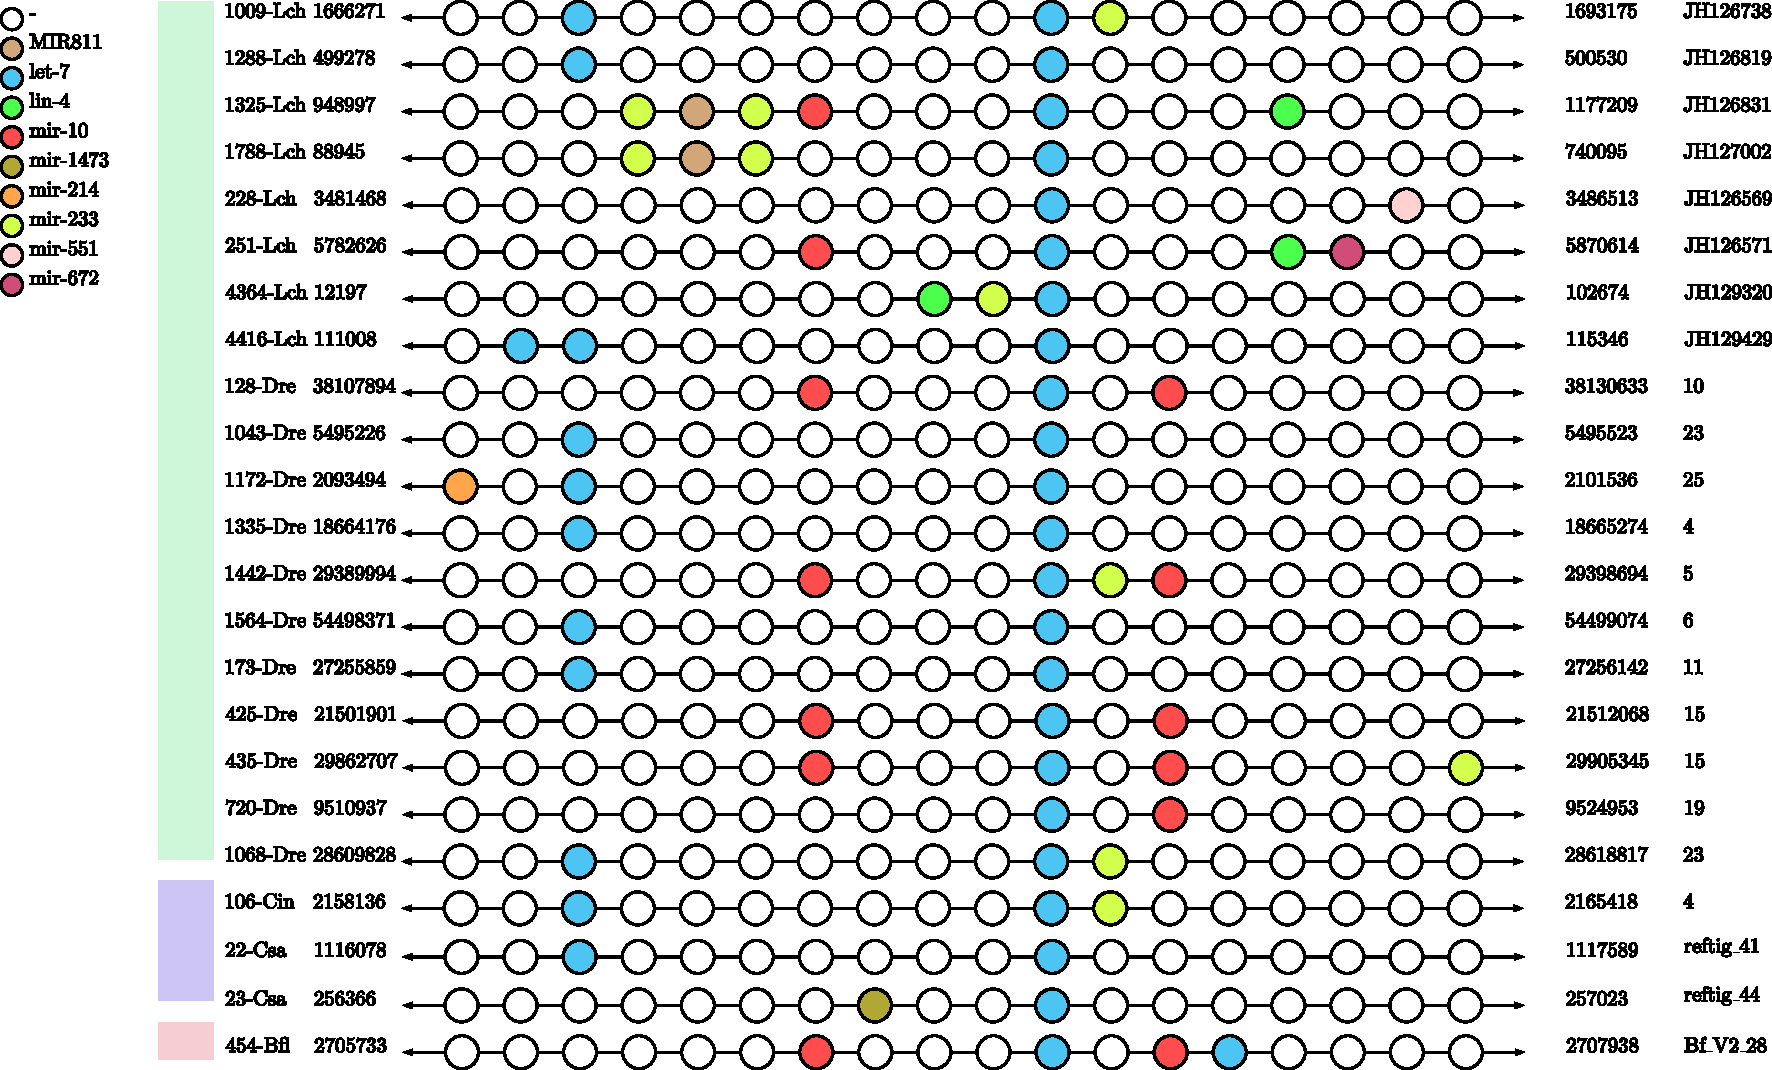
\includegraphics[width=\textwidth]{./Images/Cluster_images/let-7_101_128}
\caption{Multiple alignment of let-7 clusters. Specific names from annotations 
and homology predictions are described at the legend. Names from miRBase 
families are reported at the bottom of the aligned elements.} 
%the relationships between names and families had been found from this file:
%ftp://mirbase.org/pub/mirbase/CURRENT/miFam.dat.gz
\label{fig:let-7}
\end{figure}

\begin{figure}[ht!]
\sidecaption[t]
%\centering
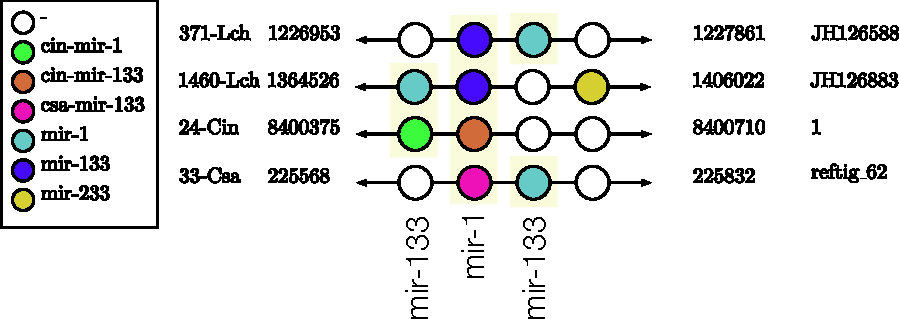
\includegraphics[width=\textwidth]{./Images/Cluster_images/mir-133_113_33}
\caption{mir-1/mir-133}
\label{fig:mir-1}
\end{figure}

\begin{figure}[ht!]
\sidecaption[t]
%\centering
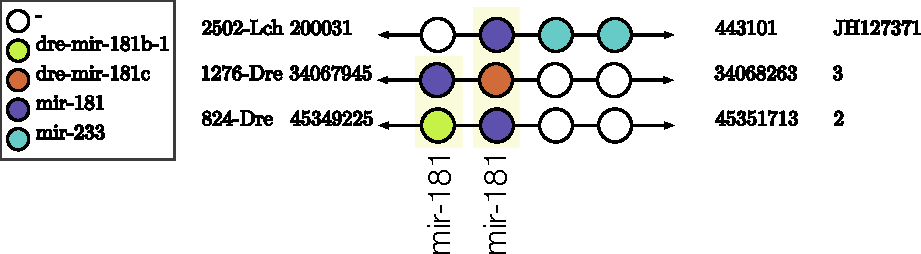
\includegraphics[width=\textwidth]{./Images/Cluster_images/mir-181_105_2502}
\caption{mir-181}
\label{fig:mir-1}
\end{figure}

\begin{figure}[ht!]
\sidecaption[t]
%\centering
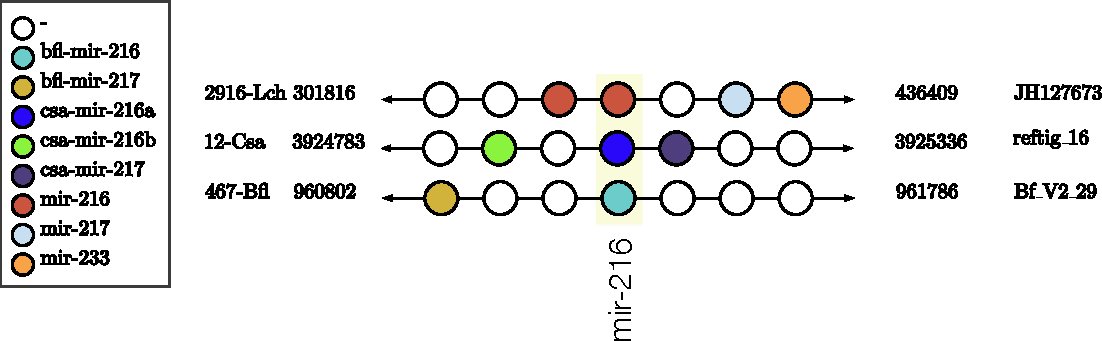
\includegraphics[width=\textwidth]{./Images/Cluster_images/mir-217_13D_467}
\caption{mir-216/mir-217}
\label{fig:mir-216}
\end{figure}

\begin{figure}[ht!]
\sidecaption[t]
%\centering
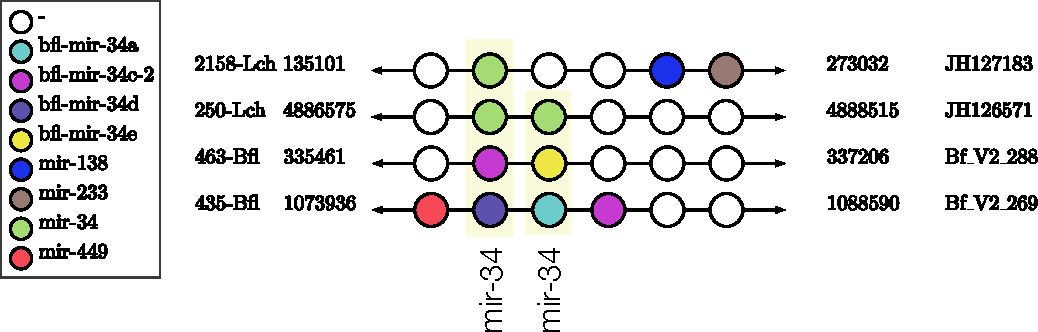
\includegraphics[width=\textwidth]{./Images/Cluster_images/mir-34_11A_435}
\caption{mir-34}
\label{fig:mir-34}
\end{figure}

\begin{figure}[ht!]
\sidecaption[t]
%\centering
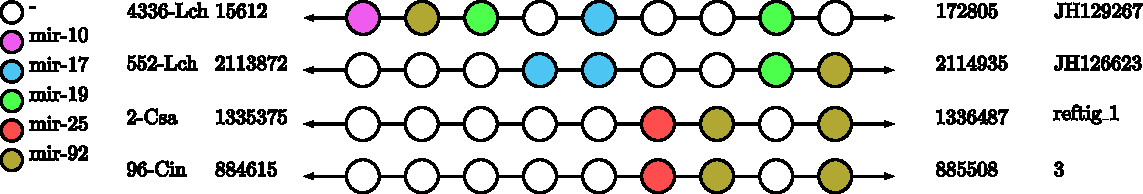
\includegraphics[width=\textwidth]{./Images/Cluster_images/mir-92_281_4336}
\caption{mir-92}
\label{fig:mir-92}
\end{figure}

\begin{figure}[ht!]
\sidecaption[t]
%\centering
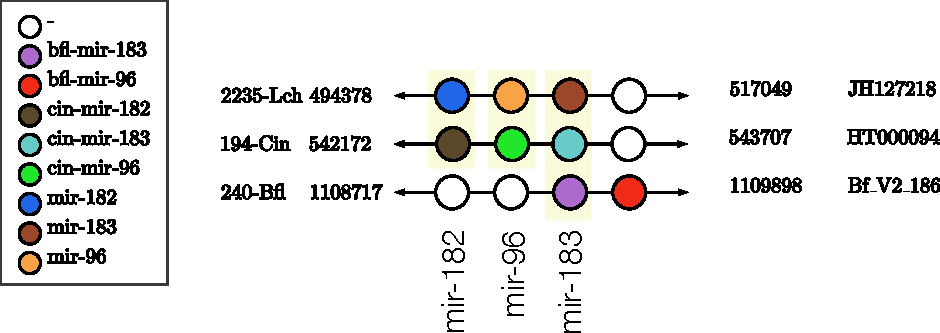
\includegraphics[width=\textwidth]{./Images/Cluster_images/mir-96_138_240}
\caption{mir-182/mir-96/mir-183}
\label{fig:mir-96}
\end{figure}

\begin{small}
\begin{center}
\begin{longtable}{clllp{2.5cm}p{3cm}p{1.5cm}p{1cm}}
\tabularnewline
\caption{Reported clusters on literature. Bold text represent those miRNAs 
elements that are currently annotated and validated, but could not 
possible to detect by homology strategies. \textbf{Ciro}: \textit{C. robusta}, 
\textbf{Cisa}: \textit{C. savignyi} and \textbf{Oidi}: \textit{O. dioica}} 
%Here I reported my calculated 
%coordinates, miRBase ones are mostly to far from Ensembl ones.}
\label{tab:otherClusters}
%\hline\noalign{\smallskip}
\tabularnewline
\cline{1-8}
\textbf{Specie} & \textbf{Chr} & \textbf{Start} & \textbf{End} 
& \textbf{miRNAs} & \textbf{Comments} & \textbf{Source DB} & 
\textbf{Ref.}\\
\tabularnewline
\cline{1-8}
Ciro & 4q & $2082260$ & $2083286$ & 
\textbf{cin-let-7a-1, cin-let-7f, cin-let-7b, cin-let-7c, cin-let-7a-2} & 
Reported on miRBAse and annotated on Ensembl & miRBase & \cite{Hendrix2010}, 
\cite{Fu2008} \\
Cisa & reftig\_41 & $1114139$ & $1117597$ & \textbf{csa-let-7c-1, 
csa-let-7b, csa-let-7a, csa-let-7c-2} & Reported on miRBase and does not 
detected by homology strategies. & miRBase & \cite{Fu2008} \\
\hline
Ciro & 10q & $3226200$ & $3228884$ & \textbf{cin-mir-34}, 
cin-mir-4091, cin-mir-4008a, cin-mir-4008c, cin-mir-4008b, cin-mir-4054 & NA & 
miRBase, Homology & \cite{Norden-Krichmar2007}, \cite{Fu2008}, 
\cite{Hendrix2010}, \cite{Terai2012}\\
\hline
Ciro & 7q & $4828431$ & $4835967$ & cin-mir-4077b, cin-mir-4003b, 
cin-mir-4005b, cin-mir-4077d, cin-mir-4003a-1, cin-mir-4003c, cin-mir-4077a, 
cin-mir-4003a-4, cin-mir-4003d & NA & miRBase, Homology & 
\cite{Hendrix2010} \\
\hline
Ciro & 3q & $567478$ & $571031$ & cin-mir-4001f, cin-mir-4000e, 
cin-mir-4001c, cin-mir-1502d, cin-mir-4018a, cin-mir-4019, cin-mir-1502b, 
cin-mir-1502a, cin-mir-4007, cin-mir-4000f, cin-mir-4001i, cin-mir-4018b, 
cin-mir-1502c & Inclusion of cin-mir-4019 and cin-mir-4007  & miRBase, 
Homology & \cite{Hendrix2010} \\ 
\hline
Ciro & HT000037.1 & $4884$ & $5250$ & \textbf{cin-mir-367}, 
\textbf{cin-mir-4009c}, \textbf{cin-mir-4009b}, cin-mir-367, cin-mir-4009c, 
cin-mir-4009a, cin-mir-4009b & Non-highlighted names could be found in the 
current genome at HT000037.1 scaffold & miRBase, Homology & 
\cite{Hendrix2010} \\
\hline
Ciro & 10q & $3226200$ & $3228884$ & \textbf{cin-mir-34}, cin-mir-4091, 
cin-mir-4008a, cin-mir-4008c, cin-mir-4008b, cin-mir-4054 & NA & miRBase, 
Homology & \cite{Hendrix2010} \\
\hline
Ciro & 3q & $884615$ & $885508$ &
cin-mir-92a, cin-mir-92d, cin-mir-92c & NA & miRBase, Homology & 
\cite{Hendrix2010} \\
Cisa & reftig\_1 & $1335375$	& $1336487$ & csa-mir-92b, 
csa-mir-92c, csa-mir-92a & NA & miRBase, Homology & \cite{Fu2008} \\
Oidi & scaffold\_1 & $3086369$ & $3086586$ & odi-mir-92b, odi-mir-92a & NA 
& Homology & \cite{Fu2008} \\
\hline
Ciro & 7q & $4969691$ & $4969912$ & cin-mir-124-1, 
cin-mir-124-2 & NA & miRBase, Homology & \cite{Hendrix2010}, \cite{Fu2008} \\
Cisa & reftig\_262 & $49392$ & $49620$ & csa-mir-124-1, 
csa-mir-124-2 & NA & miRBase, Homology & \cite{Fu2008} \\
\hline
Ciro & HT000325.1 & $8331$ & $8778$ & 
cin-mir-200, \textbf{cin-mir-3575}, cin-mir-141, \textbf{cin-mir-5611} & NA & 
miRBase, Homology &  \cite{Norden-Krichmar2007}, \cite{Fu2008}, 
\cite{Hendrix2010}, \cite{Friedlaender:12} \\
Cisa & reftig\_613 & $31353$ & $31949$ & csa-mir-200, 
csa-mir-141 & NA & miRBase, Homology & \cite{Fu2008} \\
Ciro & 7q & $4153284$ & $4156782$ & cin-mir-4006d, cin-mir-4006c, 
cin-mir-4001b-2, cin-mir-4000i, cin-mir-4006g, cin-mir-4001e, cin-mir-4001d, 
cin-mir-4000g, cin-mir-4006f, cin-mir-4000h*, cin-mir-4006b, cin-mir-4001b-1, 
cin-mir-4006e, cin-mir-4001a-1, \textbf{cin-mir-4001a-2}, cin-mir-4002, 
cin-mir-4001h, 
cin-mir-4000a-2, cin-mir-4006a-2, cin-mir-4006a-3, cin-mir-4006a-1, 
\textbf{cin-mir-4006e}, \textbf{cin-mir-4001a-1}, \textbf{cin-mir-4006b}, 
cin-mir-4000c, \textbf{cin-mir-4006e}, cin-mir-4000b-2*, 
\textbf{cin-mir-4001a-1}, cin-mir-4000b-1*, \textbf{cin-mir-4001a-2}, 
\textbf{cin-mir-4002}, cin-mir-4000d*, \textbf{cin-mir-4001h}, 
\textbf{cin-mir-4006a-3}, \textbf{cin-mir-4006a-1}, \textbf{cin-mir-4000a-1} & 
Elements marked with * are identified by homology strategies at the same 
cluster, but in another order reported by miRBase. & 
miRBase, Homology & \cite{Hendrix2010} \\
\cline{1-8}
\end{longtable}
\end{center}
\end{small}

\begin{figure}[ht!]
\centering 
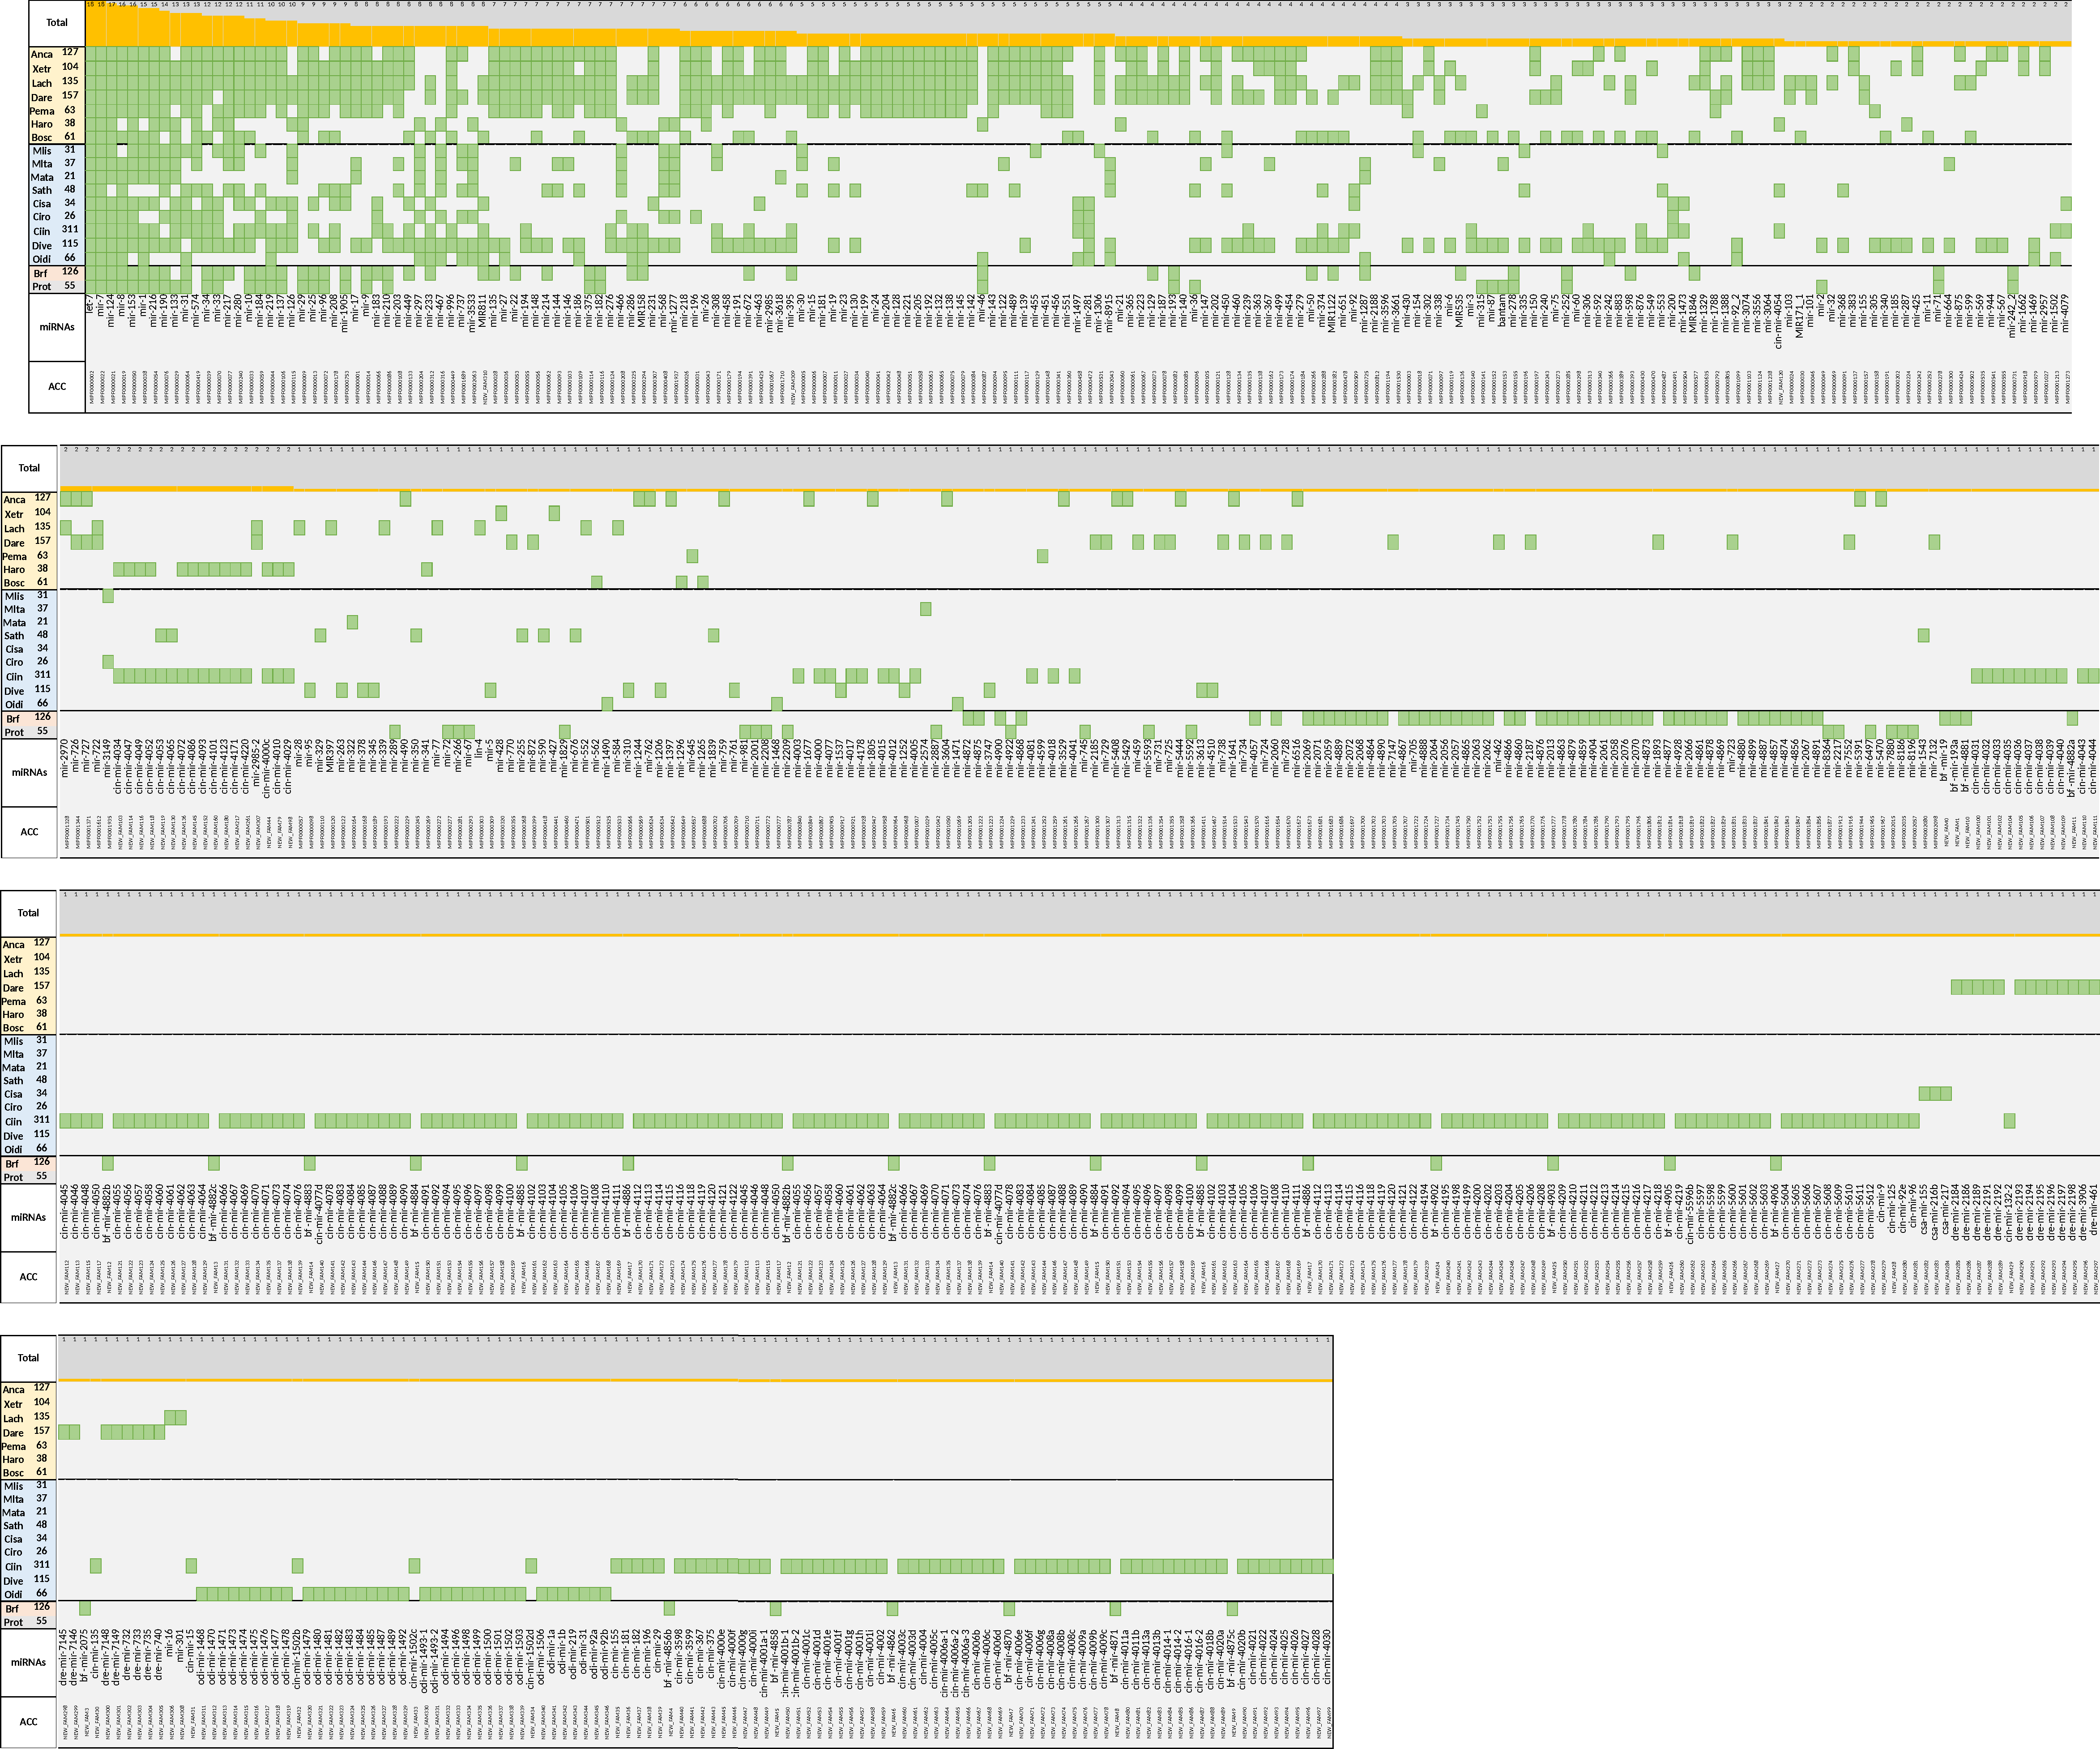
\includegraphics[width=\textwidth, angle=90]{./Images/miRNA_matrix}
\caption{Absence/Presence Matrix of miRNAs families along Bilaterian species. 
\textbf{Prot}: Protostomata, \textbf{Brfl}: \textit{B. floridae}, 
\textbf{Oidi}: \textit{O. dioica}, \textbf{Dvex}: \textit{D. vexillum}, 
\textbf{Ciin}: \textit{C. robusta}, \textbf{Cisa}: \textit{C. savignyi}, 
\textbf{Ciro}: \textit{C. robusta}, \textbf{Sath}: \textit{S. thompsoni}, 
\textbf{Mata}: \textit{M. oculata}, \textbf{Mlta}: \textit{M. occulta}, 
\textbf{Mlis}: \textit{M. occidentalis}, \textbf{Bosc}: \textit{B. schlosseri}, 
\textbf{Haro}: \textit{H. roretzi}, \textbf{Pema}: \textit{P. marinus}, 
\textbf{Dare}: \textit{D. rerio}, \textbf{Lach}: \textit{L. chalumnae}, 
\textbf{Xetr}: \textit{X. tropicalis} and \textbf{Anca}: \textit{A. 
carolinensis}. }
\label{fig:matrimirnas}
\end{figure}

\begin{figure}[t]
\sidecaption[t]
%\centering
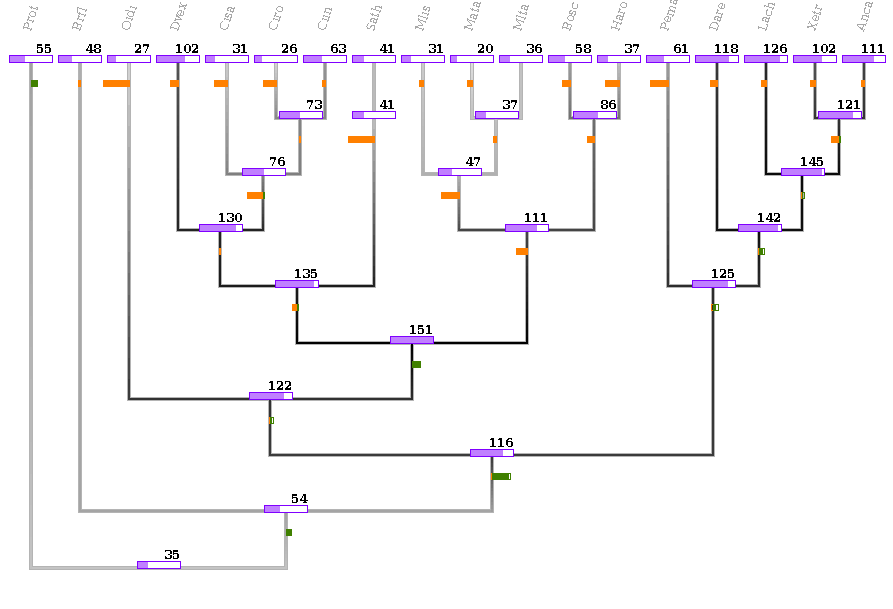
\includegraphics[width=7.5cm]{./Images/last_tree.png}
\caption{Dollo parsymony of miRNAs families distribution in some 
chordates genomes}.
\label{fig:dollotree}
\end{figure}

\begin{figure}[t]
\sidecaption[t]
%\centering
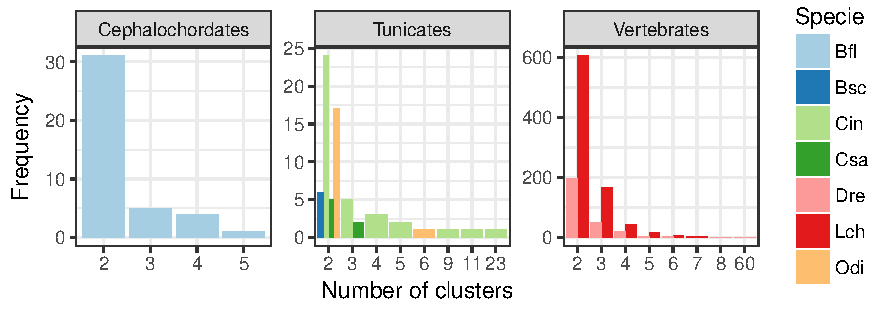
\includegraphics[width=7.4cm]{./Images/cluster_number.pdf} \\ 
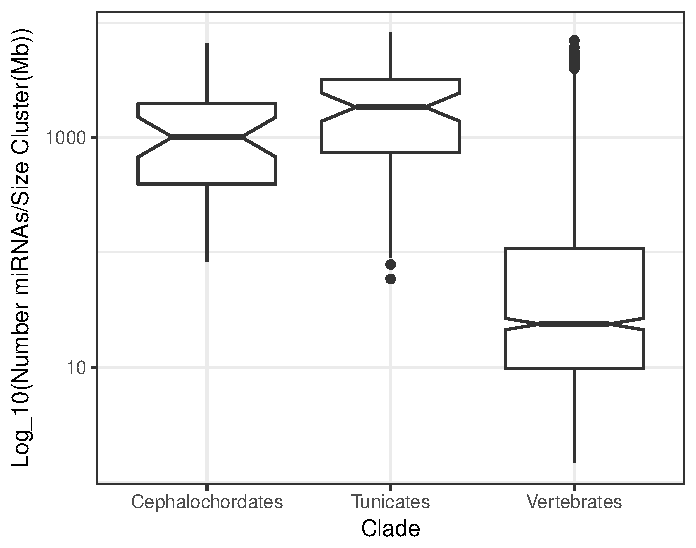
\includegraphics[width=7.4cm]{./Images/density.pdf} 
\caption{Analysis of the distribution, size and number's of cluster along 
chordate species.}
\label{fig:sizeCluster}
\end{figure}

\begin{figure}[t]
\sidecaption[t]
%\centering
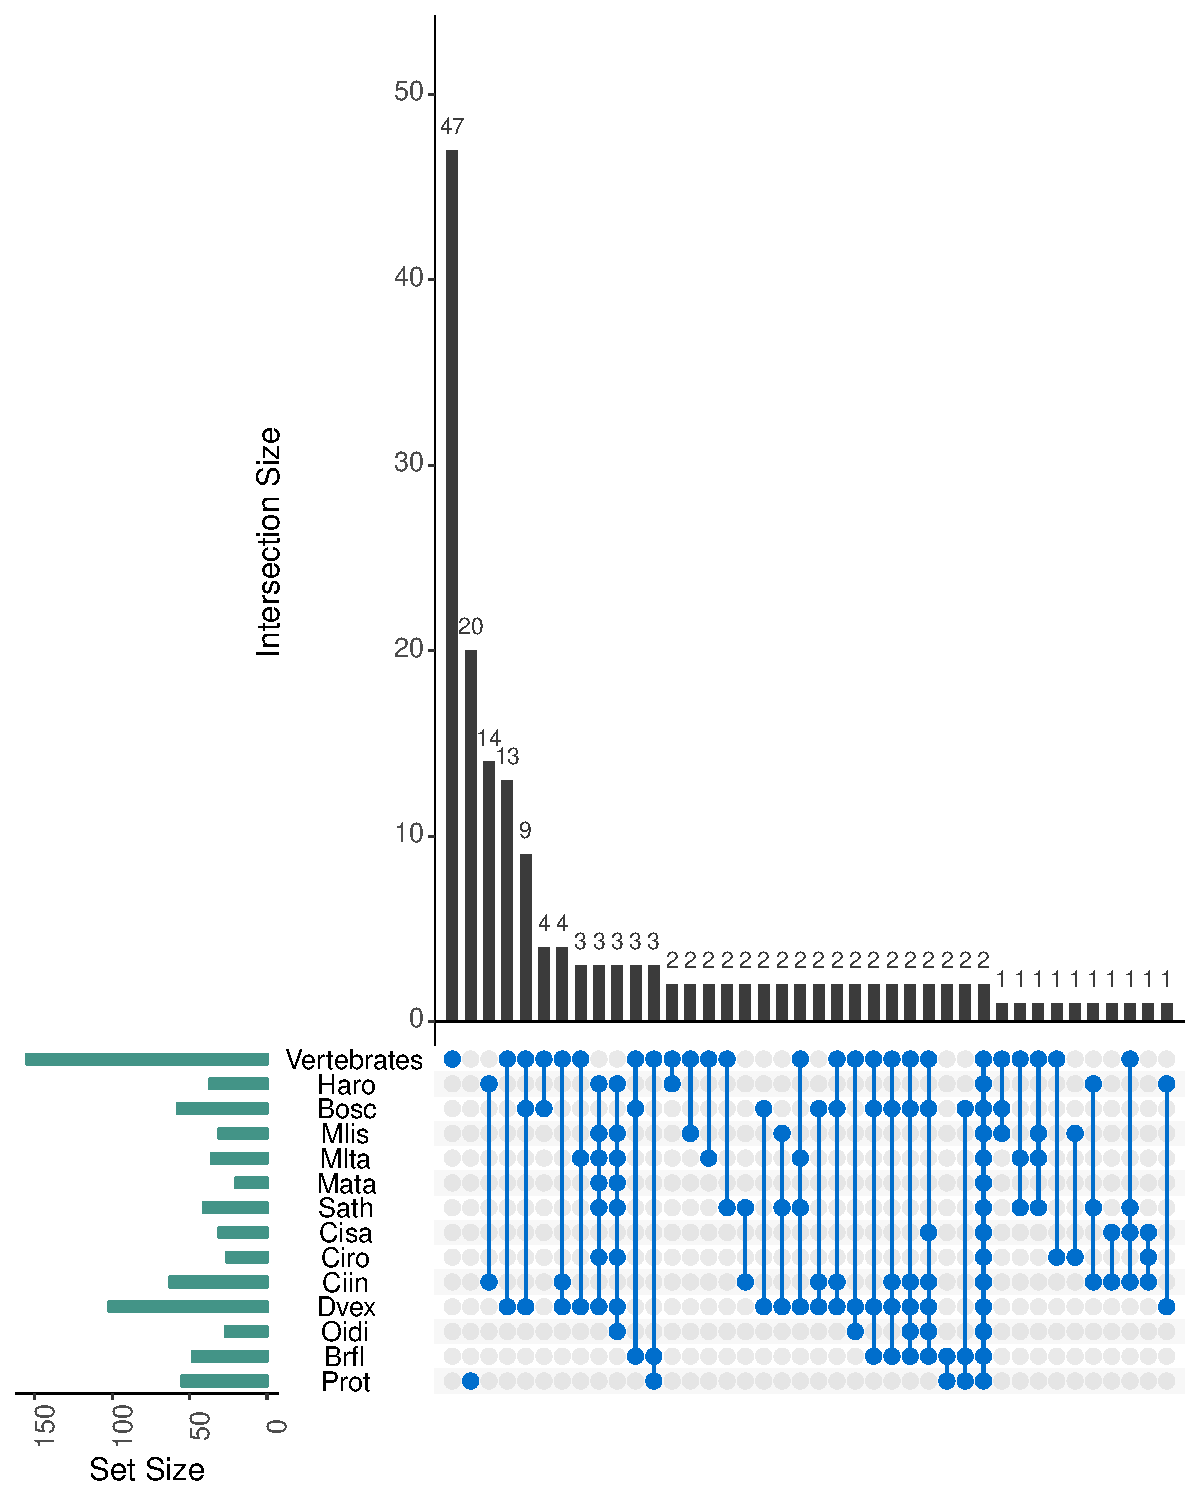
\includegraphics[width=7.5cm]{./Images/vennmiRNAs}
\caption{Comparsion between miRNAs families along Bilaterian species. Same 
labels from Figure \ref{fig:matrimirnas} were used. In this case 
\textsl{vertebrates} group the following species: \textbf{Pema}: \textit{P. 
marinus}, \textbf{Dare}: \textit{D. rerio}, \textbf{Lach}: \textit{L. 
chalumnae}, \textbf{Xetr}: \textit{X. tropicalis} and \textbf{Anca}: \textit{A. 
carolinensis}}
\label{fig:vennDiagram}
\end{figure}

\section{miRNAs and its rol in development}
\label{sec:3}

\subsection{miRNAs discovery and development}

Both MicroRNAs (miRNAs or miRs) as well as MicroRNA offset RNA (moRNAs or moRs) 
are developmentally regulated as shown during \textit{C. robusta} development 
\cite{Shi2009}. In spite of the considerably higher abundance of miRs and 
miRs* in cells than their corresponding abundance of moRs, all three small RNA 
types have been shown to have regulatory roles for gene expression. Although a 
vast majority of miRNAs remain to be studied, there are already many cases of 
well-studied miRNAs (including many that are mentioned in this chapter that 
have been studied in tunicates) that are known to target mRNAs, modulate their 
levels of expression, and affect developmental processes both in plants and 
animals \cite{Zhao2018}. Only recently two studies demonstrated for 
the first time that two moRs (viral moR-rR1-3-5p and moR-21) could also 
modulate gene expression, and were not merely the byproduct of miRNA biogenesis 
\cite{UMBACH2010592, Zhao2016}.

\subsection{Neuronal fate determination and regulation by miR-124}

The miRNA miR-124 is expressed in the nervous system of many animals, including 
Drosophila \cite{Aboobaker18017}, \textit{C. elegans} \cite{Clark:2010} and 
humans \cite{Sempere2004}. As was first observed by in vitro studies of mouse 
brain cells, low expression of miR-124 was related to neural stem cell 
maintenance, whereas high expression of miR-124 induced the differentiation of 
neuronal cell types \cite{Cheng:2009qf}. A regulative role of 
miR-124 in non-neural vs. neural fate decisions was further investigated by 
embryonic experiments in vivo \cite{Chen4943} and by 
theoretical and in silico modeling analyses in \textit{C. robusta} 
\cite{Chen2014}. These studies showed that miR-124 promotes 
nervous system development by feedback interactions with Notch signaling. 
During nervous system development of \textit{C. robusta}, cells in the dorsal 
and ventral midline epidermis of the teilbud embryo either take an epidermal 
sensory neuron (ESN) or peripheral nervous system (PNS) fate, a decision 
mediated by lateral inhibition using a classical model of feedback loop 
regulation of Notch-Delta signaling in neighboring cells \cite{Collier:1996, 
Chen2014}. Cells that take an ESN fate showed low expression of miR-124 
presumably by Notch inhibition, whereas cells that take a PNS fate expressed 
high levels of miR-124, which in the latter case it was shown to target and 
repress non-neuronal genes (e.g. neuronal repressors SCP1 and PTBP1) downstream 
of Notch signaling \cite{Chen4943}. In addition, expression 
of miR-124 in larval epidermal cells was sufficient for ectopic neural 
specification, which resembled mis-expression experiments using Pou4, an 
important transcription factor for sensory neuron specification 
\cite{Chen4943, JoyceTang2013}. Whereas miR-124 targeting to SCP1 is thought to 
have evolved in the vertebrates+tunicates, miR targeting to PTBP1 may be 
conserved among bilaterians except for ecdysozoans \cite{Chen4943} suggesting 
that the miRNA regulatory logic in lateral inhibition models of Notch-Delta 
signaling may have broader implications in other organisms yet to be studied 
\cite{Chen2014}. The research team also showed that miR-124 
acted at the gastrula stage and targeted other non-neural genes such as muscle 
determinant Macho-1 and notochord determinant Brachyury to allow for ectodermal 
fate specification \cite{Chen4943}.

\subsubsection{Muscle development and the polycistronic miR-1/miR-133 cluster}
A well-studied case of miRNA regulation in muscle development is the 
miR-1/miR-133 polycistronic cluster. Whereas miR-1 promotes differentiation of 
muscle, miR-133 promotes proliferation of muscle precursors \cite{Chen:2005yq}. 
In the chordates, these two miRNAs are encoded in an antisense direction in a 
relatively close localization (3-11 kb apart) within the gene \textit{mind bomb 
1} (MIB1), and transcribed as a single primary (i.e. polycistronic) transcript. 
Except for Drosophila and ambulacrarians (i.e. echinoderms and hemichordates), 
a close proximity of these two miRNAs has been documented in most animal taxa 
suggesting some form of functional regulatory constraint of a condensed 
miR-1/miR-133 cluster for the bilaterians \cite{Campo-Paysaa:2011}. 
During \textit{C. robusta} development, the polycistronic transcription can be 
detected in the nuclei of presumptive tail muscle cells from the gastrula stage 
onward, and its transcription is regulated by an $850$ bp sequence upstream of 
the transcipt start site \cite{Kusakabe2013}. Differential 
expression of the two miRNAs in muscle tissues was only detected in the adult, 
where body wall muscle expressed similar levels of miR-1 and miR-133 and heart 
muscle expressed significantly higher levels of miR-1 \cite{Kusakabe2013}.

\subsubsection{miRNA expression during oral siphon (OS) regeneration}
Three stages of regeneration have been proposed that reconstruct main events of 
regeneration that match expected expression profiles in the corresponding 
timeframes \cite{Knapp:2013}. The three phases correspond to: i. wound Healing, 
ii. transition, and iii. re-development. Using miRNA-mRNA transcriptional 
profiling using a correlation network, differential expression of mRNAs was 
correlated to miRNA profiles during the three regeneration windows mentioned 
above in \textit{C. robusta} oral siphon regeneration \cite{Spina:2017}. In 
the first phase, i.e. wound healing, miRNA target clusters of miR 4178b-5p and 
miR 4\_20211 were found to be correlated to the differential expression of 
genes involved in the following GO term functional classifications: immune 
response, stress response and apoptosis. In the second phase, i.e. transition, 
miR 4008c-5p, miR 4123-5p, miR 4178-5p, miR 2\_15911, miR 4\_20211, and miR 
11\_7539 were correlated and known to target Wnt, TGFb and MAPK pathway genes 
that may be regulating the proliferative state characteristic of this particular 
timeframe. In the third phase, i.e. re-development, miR4008c-5p, miR 10\_4533, 
and miR 11\_6940 known to target ECM peptidase inhibitors are correlated with 
the characteristic extracellular matrix remodeling that occurs at the final 
phase of regeneration and which resembles the original developmental processes. 
In contrast other miRs were found expressed throughout the regenerative 
process. MiRNA miR 10\_4533 known to target IGF and IGFb was found expressed 
presumably regulating the proliferation of progenitors. Also miR-9 was found 
expressed throughout regeneration and is known to be essential for neural 
development and function, presumably by targeting and regulating genes involved 
in cytoskeleton and cell cycle functions \cite{Galderisi:2003rt, 
MCBEATH2004483}, instead of targeting Notch or Hes-1 \cite{Spina:2017}.

\subsubsection{miRNA expression during \textit{O. dioica} development}
A most thorough study of the miRNA repertoire expressed during development has 
been published for the larvacean \textit{O. dioca} \cite{Fu2008}. Using a 
miRNA array approach with $55$ candidate miRNAs and $10$ developmental stages 
for analyses, some general patterns of miRNA occurrence emerged. MicroRNAs were 
expressed throughout the life cycle of the animal, and were deposited in eggs 
as maternal determinants for early zygotes. Expression of zygotic miRNAs, such 
as miR-1487 and miR-1488, was observed starting on the blastula stage (1.5h 
post fertilization). Most miRNAs analyzed showed developmental regulation (for 
specific miRNAs that were differentially expressed at each stage see 
\cite{Fu2008}), except for some such as miR-1497 that was expressed throughout 
all stages \cite{Fu2008}. From this study, the first sex specific miRNAs were 
revealed: miR-1478 was expressed day $6$ females in the oocytes, whereas 
miR-1487/88 were expressed in day $6$ males. Interestingly, the compact genomes 
of \textit{O. dioica} showed one single copy of most miRNA loci, except for 
miR-1490a, miR-1493, miR-1497d, and miR-1504 that were in two copies 
\cite{Fu2008}.


\section{Other ncRNAs associated to development}
\label{sec:4}

\subsection{Yellow Crescent RNA}

Yellow crescent RNA, i.e. YC RNA, concerns an about 1.2 kb long polyadenylated 
RNA, which can be present throughout the embryonic development of ascidians 
\cite{Swalla1995}. Its name refers to the fact that in situ hybridization 
confirmed that YC RNA is localized in the yellow crescent region of one-cell 
zygotes. The YC transcripts are actually already found in the cortex of 
unfertilized eggs, segregating with the myoplasm to the yellow crescent after 
fertilization \cite{Swalla1995}. Subsequently most YC transcripts enter the 
primary muscle cell lineage after cleavage and are also present in the 
secondary muscle cell lineage \cite{Swalla1995}. YC RNA was first 
discovered in the club tunicate Styela clava \cite{Swalla1995}. As the presence 
of the 1.2-kb RNA in oocytes and early cleaving embryos indicates that it is a 
maternal transcript, YC RNA is considered to be a maternal RNA 
\cite{Swalla1995}. It is associated with the cytoskeleton and segregates to 
the muscle cells during ascidian embryogenesis. Although the YC ORF encodes for 
a putative polypeptide of $49$ amino acids, this protein is relatively small 
and does not show any significant homology to any known proteins. As the YC RNA 
shows various features indicating that it actually functions as an RNA rather 
than as a protein coding molecule, it is considered to be a noncoding RNA that 
may play an important role in growth and development \cite{Swalla1995}.

\subsection{MicroRNA-offset RNAs}

MicroRNA-offset RNAs, i.e. moRNAs, concern about $20$ nucleotides long RNAs 
that lie adjacent to pre-miRNAs. They can originate from both ends of these 
pre-miRNAs, although prevalently they are derived from the 5' arm 
\cite{bortoluzzi2011}. During a study focused on identifying miRNAs in the 
simple chordate \textit{C. robusta} moRNAs were first discovered 
\cite{Shi2009}. Unexpectedly, half of the \textit{C. robusta} miRNA loci 
that were detected in this study turned out to encode for 
previously uncharacterized small RNAs, in addition to conventional miRNA and 
miRNA* products. This new class of RNAs was hereafter referred to as `moRNAs', 
for miRNA-offset RNAs. It became clear that these moRNAs are probably produced 
by RNAse II-like processing and are observed, like miRNAs, at specific 
developmental stages \cite{Shi2009}.
These results and subsequent studies gave rise to the hypothesis that moRNAs 
concern  a new class of functional regulators whose qualitative alteration 
and/or expression dysregulation might even impact human diseases 
\cite{bortoluzzi2011}. Evidence supporting this hypothesis is still fragmentary 
however. After the discovery in \textit{Ciona}, moRNAs were 
also found in human cells by deep sequencing analysis. Hereby it was reported 
that moRNAs from $78$ genomic loci were weakly expressed in the prefrontal 
cortex \cite{Langenberger2009}. Additional indications that moRNA have a 
distinct function include the fact that some moRNAs are as conserved as miRNAs 
and are in fact conserved across species to an extent that correlated with 
expression level \cite{Shi2009}. The expression level of certain moRNAs can 
even be greater than for their corresponding miRNA \cite{Umbach2010}. Finally, 
it can be argued \cite{bortoluzzi2011} that it is likely that moRNAs might 
represent a functional class of miRNA-related agents as moRNAs are prevalently 
produced by the 5' arm of the precursor, independent of which arm produces the 
most expressed mature miRNA \cite{Langenberger2009, Umbach2010}. 
What functions moRNAs may have, varies. For example, moRNA expression was 
recorded in solid tumours, together with other small RNAs \cite{Meiri2010}. 
In addition the fact that an 18-fold enrichment of moRNAs was observed in the 
nucleus \cite{Taft2010} indicates that at least some moRNAs may have functions 
related to nuclear processes \cite{bortoluzzi2011}. Recently, an specific class 
of moRNAs (moRNA-21) has been associated with post-transcriptional gene 
regulation, proliferation of vascular smooth muscle cells (VSMC) and mediated 
gene down-regulation in a process mediated by Ago2 \cite{Zhao2016}. Although 
these studies do provide good indications, the potential functional roles that 
moRNAs can play, remain still largely unknown.

\subsection{Long Noncoding RNA RMST}

Long noncoding RNAs, i.e. lncRNAs, are abundantly found within mammalian 
transcriptomes. One of the known groups of lncRNAs, includes the 
rhabdomyosarcoma 2-associated transcript (RMST), which is indispensable for 
neurogenesis \cite{Bogu2013}. 
Human RMST was shown as being responsible for the modulation of neurogenesis as 
its expression is regulated by the transcriptional repressor REST while it 
increases during neuronal differentiation \cite{Bogu2013}. Hereby it was 
found that RMST is actually necessary for the binding of SOX2 to promoter 
regions of neurogenic transcription factors. SOX2, a transcription factor known 
to regulate neural fate, in combination with RMST were actually found to 
coregulate a large pool of downstream genes implicated in neurogenesis, i.e. 
more than $1\,000$ genes were differentially expressed upon RMST knockdown 
\cite{Bogu2013}. These results illustrated the role of RMST as a 
transcriptional coregulator of SOX2 and a key player in the regulation of 
neural stem cell fate \cite{Bogu2013}. A further confirmation of the importance 
of RMST came with the discovery of a homologue of this lncRNA in the simple 
chordate \textit{D. vexillum}, i.e. the carpet sea-squirt 
\cite{Velandia-Huerto2016}. While homologues of ``human'' lncRNAs are 
rarely found across all chordates due to their low levels of sequence 
conservation, a plausible homolog of RMST $9$, the conserved region $9$ of the 
Rhabdomyosarcoma 2 associated transcript known for its interaction with SOX2, 
was found in \textit{D. vexillum}. Subsequently putative homologs were also 
found in the genomes of the ascidians \textit{C. robusta}, \textit{C. 
savignyi} and \textit{B. schlosseri} and the Florida lancelet \textit{B. 
floridae}, illustrating that RMST lncRNA are thus conserved across chordates, 
making them one of the best conserved lncRNAs known to date 
\cite{Velandia-Huerto2016}.

\subsection{Splices-leader RNA}

mRNA 5'leader trans-splicing is a mode of gene expression in which the 5' end 
of a pre-mRNA is discarded and replaced by the 5' segment of a spliced leader 
(SL) RNA \cite{Vandenberghe2001}. Spliced-Leader RNAs, i.e. SL RNAs, hereby 
consist of a 5' exon and a 3' intron with a conserved consensus 5' splice donor 
site at the exon-intron boundary \cite{Ganot2004}. SL RNA trans splicing has 
not only been described for euglenoids, kinetoplastids, cnidarians, nematodes, 
and Platyhelminthes \cite{Ganot2004}, but also for deuterostomes like the 
simple 
chordate \textit{C. robusta} \cite{Vandenberghe2001} and the 
appendicularian \textit{O. dioica} \cite{Ganot2004}. Hereby \textit{O. dioica} 
was shown to not only trans-splice SL RNAs to mRNAs, as does \textit{C. 
robusta}, but also to use trans splicing in resolving polycistronic 
transcripts \cite{Ganot2004}. During trans splicing, the capped SL RNA exon 
moiety is covalently linked to the 5' ends of mRNAs, forming a leader sequence 
ranging from $16$ nt in \textit{C. robusta} to $41$ nt in trypanosomatids 
\cite{Ganot2004}. The role of SL trans-splicing is still unknown in many cases. 
SL trans-splicing may potentially having functions varying from the mediation 
of mRNA stability or translatability \cite{Maroney1995} and the resolution 
of polycistronic pre-mRNAs \cite{Agabian1990, Blumenthal1995}, to the 
production of functional mRNAs from RNA polymerase I 
transcripts \cite{ShuLee1997}.

\section{Acknowledgments}
This work and the computational analysis were partially supported by the 
equipment donation from the German Academic Exchange Service-DAAD to the 
Faculty of Science at the Universidad Nacional de Colombia. Also, by the 
computational laboratory from Bioinformatics Group at Department of Computer 
Science and Interdisciplinary Center for Bioinformatic at the Leipzig 
University. The comparative analysis was partially supported by Colciencias 
(project no.\ 110165843196, contract 571-2014). CAVH acknowledges the support by 
DAAD scholarship: Forschungsstipendien-Promotionen in Deutschland, 2017/18 
(Bewerbung 57299294). CIBS acknowledges Universidad Nacional de Colombia for the 
time granted to write this chapter.

% BibTeX users please use
\bibliographystyle{plain}
\bibliography{tuni_updated}
%\bibliography{tuni, tuni_2, Arjan/biblio_arjan}
%%%%%%

\end{document}
